% !TeX TXS-program:compile = txs:///pdflatex/[--shell-escape]
% Le truc au-dessus pour avoir l'option shell-escape qui permet de faire du minted.
\documentclass[12pt]{article}

% Affichage ou non des reponses aux questions & exercices
\newif\ifDispRep
%\DispReptrue  % Show the text
\DispRepfalse % Hide the text

% Version du document
\newcommand{\versiondoc}{v0.1}

% Incorporation tous éléments de préambule communs à tous mes cours
% Sans chemin relatif parce que TexStudio lancé depuis un script qui prend en compte la variable d'environnement TEXINPUTS
\usepackage{CoursLFC}

% Eléments de l'en-tête et de la page de garde spécifiques à ce doc
\newcommand{\classe}{1\textsuperscript{ère} NSI}
\newcommand{\themecours}{Thème 6: Algorithmique}
\newcommand{\datedoc}{février 2024}

% Page de garde mise en page
\title
	{\vspace{3cm}
		{\Large
		\textit
			{
				\classe\hspace{0.1cm}
				\textemdash\
				\hspace{0.1cm}
				\themecours
			}
			
		\vspace{1cm}
		\huge{Algorithmique \& Mise au Point de Programmes} }
		 
		\vspace{1cm}
	}
\author{\etablissement}
\date{
	\auteur,
	\datedoc,
	\footnotesize{\textit{\versiondoc}} 
	\vspace{6cm}
	}

% Header & Footer
\lfoot{\etabshort}
\cfoot{\thepage}
\rfoot{\classe, \anneescol}
\renewcommand{\footrulewidth}{0.2pt}
\lhead{}
\chead{}
\rhead{}
\renewcommand{\headrulewidth}{0pt}

\begin{document}
	
	\maketitle
	% pas de footer sur la première page
	\thispagestyle{empty}
		
	\section*{}
		{\noindent
		\resumecours
		}
		
	\pagebreak	
	\tableofcontents
	
	\pagebreak
	
	% Début du contenu du document

	\section{Point d'étape -- où est-on / où va-t-on?}
	\subsection{Ce qu'on a couvert jusqu'à présent}
	
	\begin{itemize}
		\item Rudiments de l'architecture physique d'un ordinateur -- le modèle de Von Neumann.
		\item Mise en jambes sur de l'écriture de code: réalisation d'une page Web en HTML.
		\item Introduction à Python, et plus spécifiquement:
		\begin{itemize}
			\item Ce qu'on appelle ses "constructions élémentaires" -- variables, fonctions, conditions \& embranchements, boucles...
			\item Les types et valeurs de base: entiers (naturels et relatifs), flottants (réels), chaînes de caractères et booléens (qu'on n'a que brièvement abordés pour l'instant).
			\item Un type dit "construit" -- les listes.
		\end{itemize}
		\item Un peu de théorie: la représentation des types et valeurs de base en machine (les entiers naturels et relatifs, les réels, les alphanumériques).
		\item Un peu plus de théorie: introduction à la logique booléenne (que l'on n'a couverte que très rapidement -- on y reviendra en fin d'année).
		\item Un retour à la pratique: le traitement de données en table, la manipulation de fichiers dans Python, et des types de données plus complexes --- les dictionnaires, les listes de dictionnaires...
	\end{itemize}
	
	\subsection{Ce dont on va parler dans ce nouveau chapitre}
	On a donc fait des "sauts" de la théorie vers la pratique, puis vers la théorie de nouveau --- pour finalement atterrir ici, dans ce chapitre sur l'algorithmique qui se trouve presque exactement au "milieu" de cet axe théorie--pratique.
	
	Comme je vous l'ai dit à plusieurs reprises dans les parties précédentes -- et spécialement dans celle portant sur le traitement de données en table, l'algorithmique, vous en faites déjà: je vous pose des problèmes par le biais de notebooks Jupyter dans Capytale v2 et vous réfléchissez à comment les résoudre. Dit autrement, \textit{vous concevez des algorithmes}.
	
	Ce que l'on va faire dans ce nouveau chapitre c'est formaliser cette démarche, la structurer, puis étudier quelques exemples d'algorithmes beaucoup plus avancés que ce que l'on a vu jusqu'à présent.
	
	Spécifiquement, on va parcourir le chemin suivant:
	\begin{itemize}
		\item Introduction à l'algorithmique -- étapes de conception et de rédaction d'un algorithme;
		\item Pratique: tests d'algorithmes / de programmes;
		\item Preuve d'algorithmes;
		\item Complexité d'algorithmes;
		\item Etude de certains algorithmes spécifiques:
		\begin{itemize}
			\item Algorithmes de tri - par sélection, par insertion;
			\item Algorithme de recherche dichotomique dans un tableau;
			\item Algorithmes gloutons;
			\item Algorithmes des k plus proches voisins -- algorithme d'apprentissage, "machine learning".
		\end{itemize}
		\item Pratique: mise au point de programmes; programmation défensive.
	\end{itemize}
	
	\subsection{Comment on va procéder}
	Comme dit plus haut, on est ici à la frontière entre la théorie et la pratique -- on va donc avoir un fonctionnement hybride en classe:
	 \begin{itemize}
	 	\item \textbf{Prise de notes essentielle} --- vous commencez à connaître les cours que je vous fournis, il sont \textit{très} longs. Ils doivent vous servir de référence, vous permettre surtout de bien revoir les corrections d'exercices, mais votre savoir, lui, doit venir de votre prise de notes;
	 	\item Plusieurs exercices sur papier qu'on fera en classe et dont il sera très important que vous gardiez une trace;
	 	\item En parallèle et en complément, quelques applications / exercices sur machine.
	 \end{itemize}
	 
	 \pagebreak
	 
	 \section{Introduction à la conception d'algorithmes}
	 
	 Quelques questions pour commencer...
	 
	 \MaQuest{Qu'est-ce qu'un algorithme (indice: c'est constitué de trois parties)? }
	 \begin{MaReponse}
	 	Un algorithme est une \textbf{suite finie d'instructions} permettant de \textbf{résoudre un problème}. Il est structuré en trois parties:
		 \begin{alphenum}
		 	\item L'entrée des données;
		 	\item Le traitement des données;
		 	\item La sortie des données 
		 \end{alphenum}
	\end{MaReponse}
	
	\MaQuest{Parmi les éléments suivants, qu'est-ce qui est un algorithme, qu'est-ce qui n'en est pas?
		\begin{alphenum}
			\item Une recette de gâteau au chocolat;
			\item La liste des présidents de la V\textsuperscript{ème} République;
			\item Les règles du jeu d'échecs;
			\item Les règles à appliquer pour résoudre une équation du 2\textsuperscript{nd} degré;
			\item Les instructions de montage d'un meuble Ikea.
		\end{alphenum}
	}
	
	\begin{MaReponse}
		\begin{alphenum}
			\item Oui c'en est un -- ingrédients en entrée, étapes de confection, gâteau en sortie. C'est bien la résolution d'un problème (en l'occurrence "comment fabriquer un gâteau au chocolat?").
			\item Non ce n'en est pas un -- c'est une liste d'informations, pas des étapes à suivre.
			\item Ce n'en est pas un non plus -- ce n'est qu'une liste de principes. En revanche on pourrait les utiliser pour mettre en \oe{}uvre un algorithme qui joue aux échecs (et résoud le problème "comment jouer -- et gagner -- une partie d'échecs?).
			\item Oui c'en est un -- c'est même écrit dans la description ("résoudre").
			\item Oui c'en est un également.
		\end{alphenum}
	\end{MaReponse}
	
	\begin{MonAmp}{Définition}
		L'algorithmique est:
		\begin{itemize}
			\item La conception (et la production) d'algorithmes;
			\item Leur étude -- leur analyse, la mesure de leur fiabilité (est-ce qu'il répond vraiment au problème posé?) et de leur efficacité (est-ce qu'il le fait en un temps acceptable?).
		\end{itemize}
	\end{MonAmp}
	
	Nous allons dans ce cours nous intéresser à ces deux composantes, en commençant, dans ce chapitre, par la première dont les étapes peuvent se résumer ainsi:
	\begin{enumerate}
		\item Énoncé d'un problème à résoudre;
		\item Spécification de l'algorithme -- nom, entrées, sorties;
		\item Explicitation de la démarche en pseudo-code -- description du traitement des données qui va permettre de résoudre le problème;
		\item Traduction en langage de programmation.
	\end{enumerate}
	
	La 1\textsuperscript{ère} et la 4\textsuperscript{ème} étape sont à la marge de notre propos ici:
	\begin{itemize}
		\item L'énoncé d'un problème à résoudre par le biais d'un programme informatique est une activité à part entière (souvent appelée "expression de besoin" dans le monde professionnel). Vous y avez un petit peu touché dans le cadre de vos projets, mais dans l'ensemble, dans le contexte de la NSI, les problèmes vous sont posés -- et votre rôle consiste à savoir les résoudre;
		\item La traduction en langage de programmation, que dans le contexte de la NSI nous réalisons en Python, a fait l'objet d'un pan du cours distinct; nous allons évidemment y revenir en partie ici, mais la syntaxe Python n'est pas l'objet de notre étude ici.
	\end{itemize}
	
	\subsection{Écrire un algorithme: spécification}
	
	Avant d'écrire un algorithme il faut bien définir ce que l'on veut faire et à partir de quoi; il s'agit de donner \textbf{une spécification au problème}. Pour cela on doit:
	\begin{itemize}
		\item Donner un nom explicite à l’algorithme --- \textit{par exemple \texttt{CuissonGateauChocolat}};
		\item Décrire les conditions d'utilisation de l'algorithme, les données qu'il attend en entrée et les conditions dans lesquelles il va pouvoir être exécuté, sa \textbf{\textit{précondition}} --- \textit{par exemple "\texttt{Beurre et Lait non périmés}"}:
		\item De même, décrire le résultat attendu, sa \textbf{\textit{postcondition}}, la nature des données renvoyées et à quoi elles correspondent --- \textit{par exemple "\texttt{gâteau rond, moelleux, et succulent}"}.
	\end{itemize}
	
	Cette étape de spécification est fondamentale -- c'est en quelque sorte la "carte d'identité" de notre algorithme, ce qui va permettre à quelqu'un qui ne le connait pas de le comprendre sans avoir besoin de lire son code. On va donc la transcrire dans notre code Python en tête de la fonction lui correspondant -- et c'est exactement ce que je vous demande de faire dans vos projets.
	
	\begin{MonAmp}{Méthode}
		La transcription de la spécification d'un algorithme en tête de la fonction Python lui correspondant s'appelle "\textit{\textbf{le docstring}}" ou "\textit{\textbf{la documentation}}" de la fonction. Il est inscrit entre deux séries de trois apostrophes -- par exemple:
		\MonPython{001_Docstring.py}
	\end{MonAmp}
	
		\begin{MonExo}[Rédaction d'une spécification de fonction]
		Considérez la fonction suivante:
		\MonPython{002_MedianeNoDocstring.py}
		
		Est-ce que ce qu'elle fait est clair d'entrée de jeu? 
		
		Rédigez la docstring de cette fonction pour remédier à cela.
	\end{MonExo}
	
	\begin{MaReponse}
		On aura noté deux problèmes ici -- l'absence de docstring, mais également l'absence d'un nom explicite à la fonction ("Fonction", ce n'est franchement pas génial...). Remédions à tout cela:
		\MonPython{003_MedianeDocstring.py}
		Vous remarquerez l'inclusion d'exemples dans la docstring -- il ne faut surtout pas hésiter à y recourir, c'est ce qu'il y a de plus parlant pour quelqu'un qui découvre votre code!
	\end{MaReponse}
	
	\subsection{Ecrire un algorithme: pseudo-code}

	Si l'on se réfère aux étapes listées plus haut, on en est maintenant au moment où l'on sait \textit{ce que va réaliser} notre programme, \textit{ce qu'il va prendre en entrée}, et \textit{ce qu'il va retourner en sortie}. Il s'agit à présent d'expliciter le \textit{\textbf{comment}} -- quelles sont les étapes qui vont être effectuées pour résoudre le problème? Quel traitement va-t-on appliquer aux données en entrée pour produire les données en sortie?
	
	On a déjà utilisé à de multiples reprises le pseudo-code dans ce cours -- donc (\textit{en théorie}) vous devriez déjà être convaincus de son intérêt et savoir l'utiliser. Nous allons donc passer directement à quelques exercices d'application -- en rappelant tout de même au préalable les principes et règles suivants:
	\begin{alphenum}
		\item Le pseudo-code est une façon de décrire un algorithme pour qu'il soit compréhensible "entre humains".
		\item Le pseudo-code est indépendant du langage de programmation -- un algorithme convenablement écrit devrait en théorie pouvoir être implémenté aussi aisément en Python qu'en C ou qu'en JavaScript\footnote{C'est évidemment un peu simpliste d'écrire ceci ainsi, mais en théorie le principe est vrai: lorsque vous rédigez un algorithme en pseudo-code, vous devriez ne pas avoir de langage de programmation spécifique en tête.}. A titre d'exemple, voici un "Hello World" en deux langages de programmation distincts, mais partant du même pseudo-code:
		\begin{figure}[ht]
			\centering
			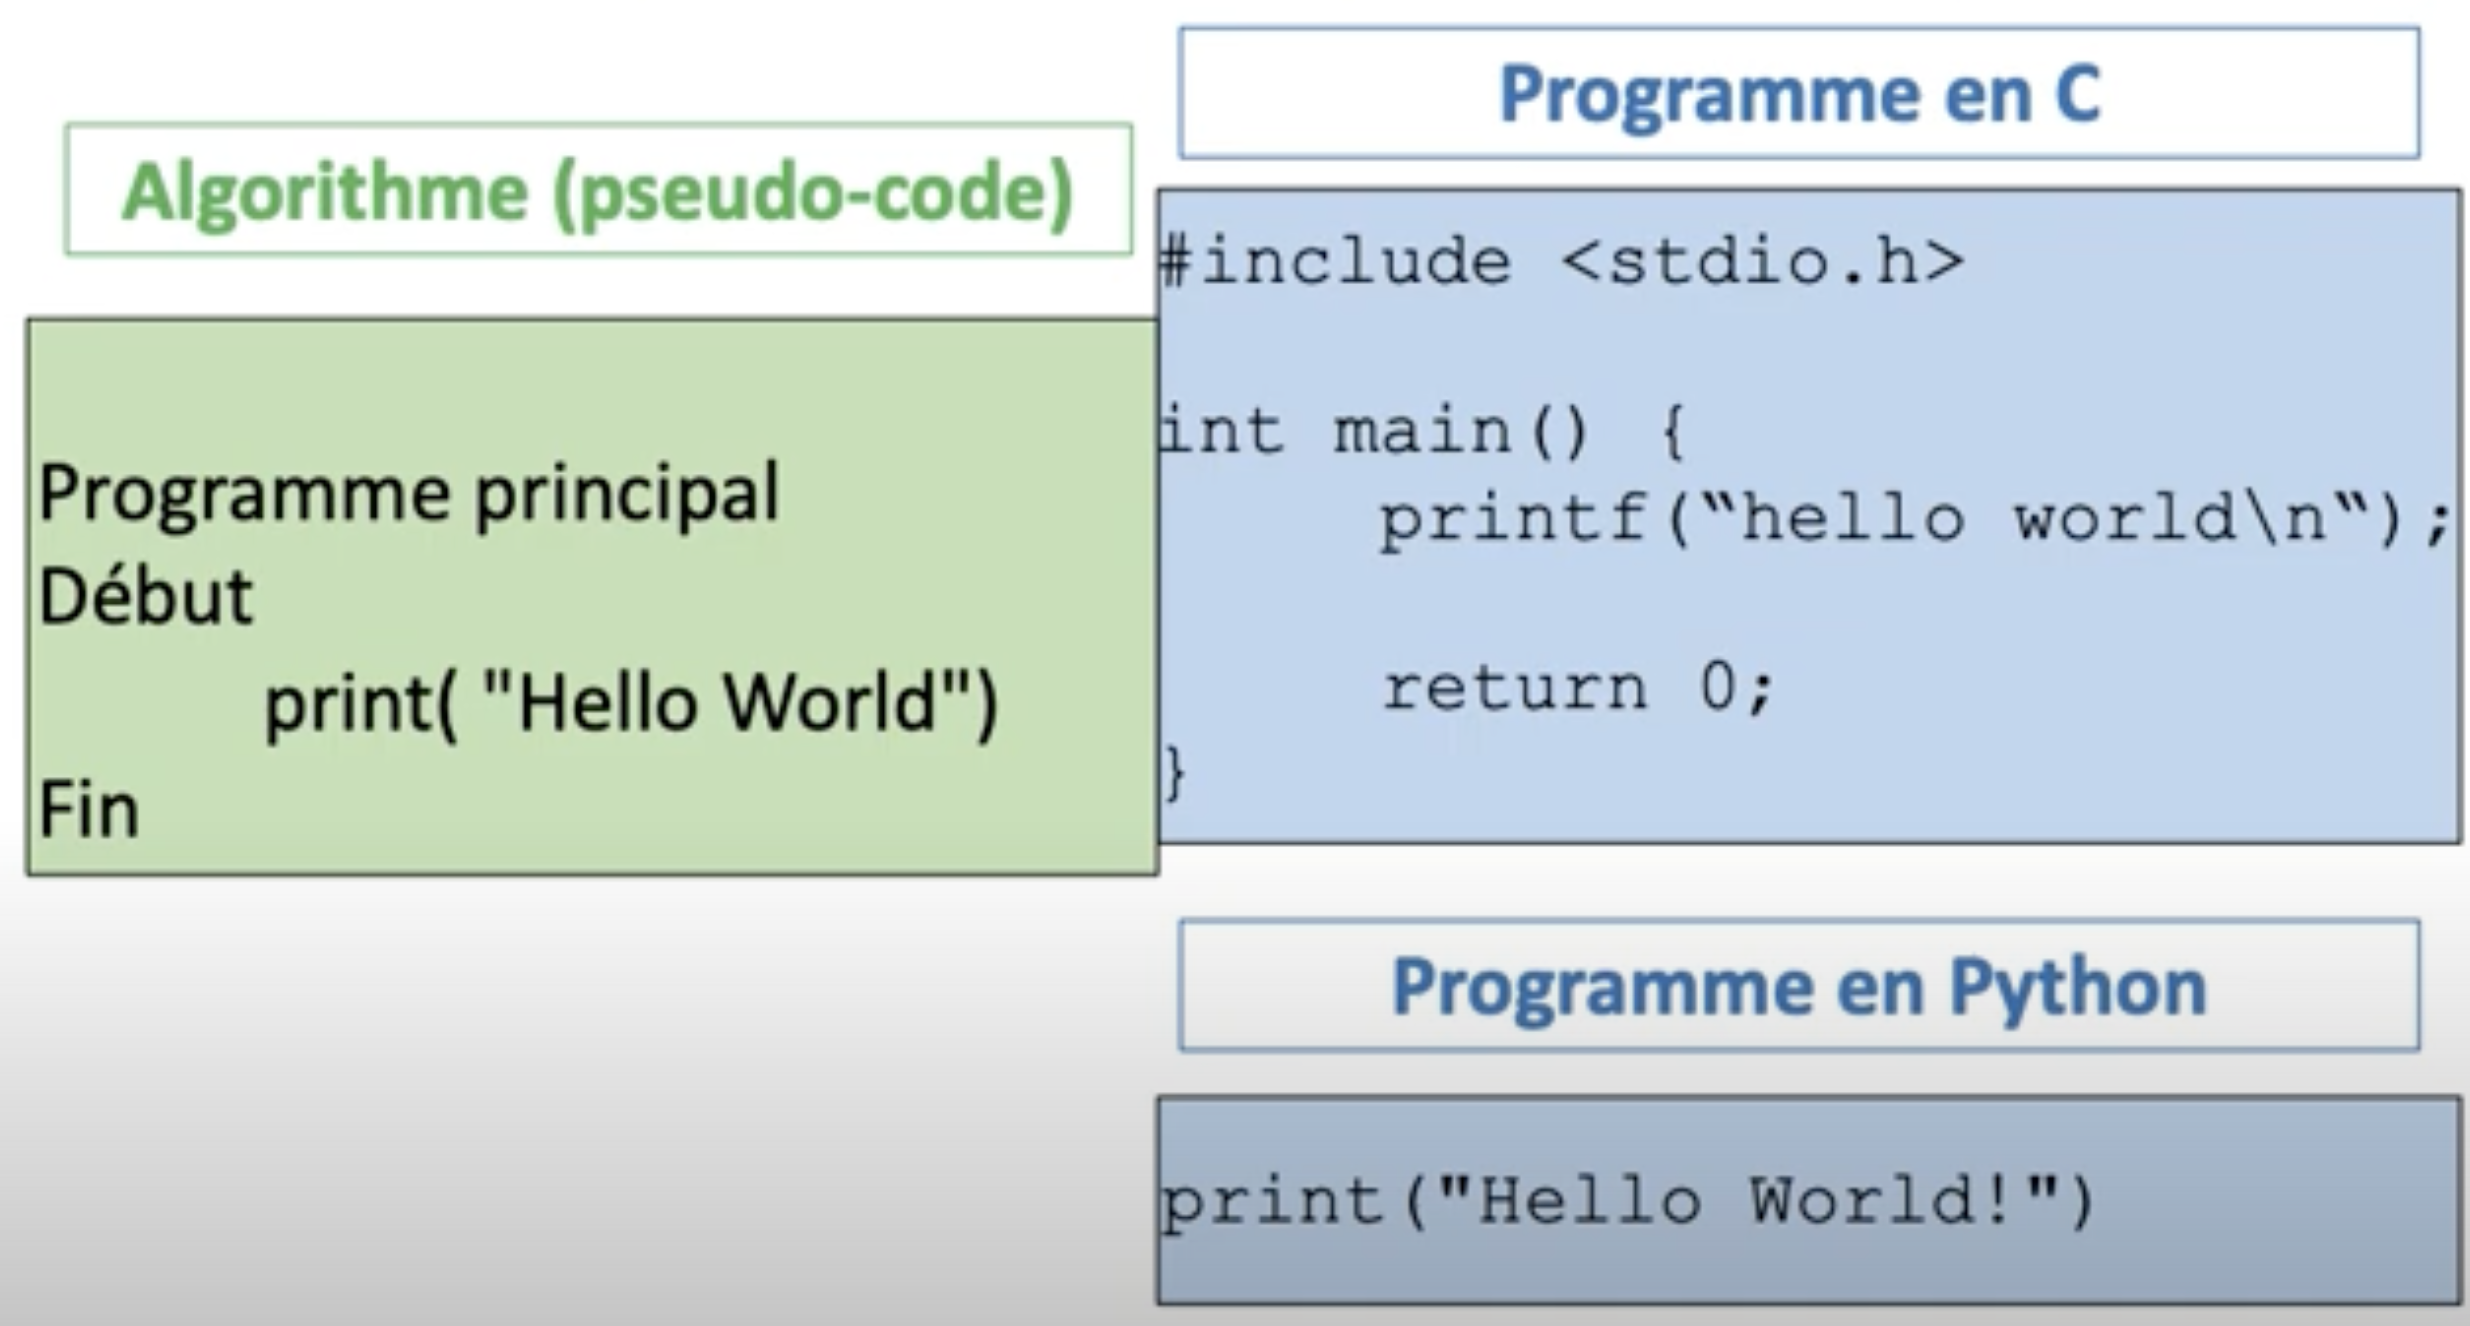
\includegraphics[width=0.5\textwidth]{001_AlgoHelloWorld.png}
		\end{figure}
		\item Conséquence: les règles de syntaxe de pseudo-code sont inspirées des éléments communs à la plupart des langages de programmation.
		\item Il n'y a pas de pseudo-code universel -- le seul principe à respecter, c'est que les règles de syntaxe appliquées soient bien définies, comprises et partagées par tous$\cdot$tes celles et ceux qui seront amené$\cdot$e$\cdot$s à lire les algorithmes.
	\end{alphenum}
	
	Ce dernier point implique qu'il y ait quand même une ossature de règles minimales dans un contexte donné -- comme pour ce cours par exemple:
	\begin{MonAmp}{Règles pseudo-code 1\textsuperscript{ère} NSI}
		\begin{alphenum}
			\item On spécifie explicitement en début d'algorithme les entrées attendues et les sorties prévues;
			\item On utilise une flèche vers la gauche ("$\leftarrow$" ou "$\lhd$") pour affecter des variables;
			\item On utilise l'indentation pour délimiter les fonctions, les conditions, les boucles...\footnote{Ici on triche un peu puisque l'indentation est spécifique à Python -- mais pas tant que ça puisque cela restera compréhensible même pour une implémentation dans un autre langage.}
			\item On explicite la fin de toute structure (fonction, condition, boucle...) débutée;
			\item On n'hésite pas à inclure des commentaires pour expliquer les étapes -- et dans ce cas, on les préfixe d'une flèche vers la droite ("$\rightarrow$" ou "$\rhd$")
			\item ... et c'est tout!
		\end{alphenum}
	\end{MonAmp}	 
	
	Pour illustrer ces principes, voici le pseudo-code d'une fonction (qu'on a déjà vue dans un chapitre précédent, d'ailleurs) prenant une liste de réels positifs en entrée et qui en renvoie le maximum:
	
	\vspace{\baselineskip}
	
	\begin{algorithmic}[1]
		\Require{$liste$ dont tous les éléments $\in \mathds{R+}$}
		\Ensure{$Max \in \mathds{R+}$}
		\Function{TrouveMax}{liste}
		\State Max $\leftarrow$ 0
		\ForAll{$Element$ de liste}
		\If{$Element > Max$}
		\Comment{On a trouvé un nouveau max}
		\State $Max$ $\leftarrow Element$
		\EndIf
		\EndFor
		\State\Return{$Max$}
		\EndFunction
	\end{algorithmic}
	
		\begin{MonExo}[Rédaction d'algorithmes en pseudo-code]
		En appliquant les principes énoncés ci-dessus, rédigez les algorithmes suivants:
		\begin{alphenum}
			\item Un algorithme qui prend deux nombres en entrée et affiche leur somme.
			\item Un algorithme qui calcule la somme des N premiers entiers naturels.
			\item Un algorithme qui génère les N premiers termes de la séquence de Fibonacci. (rappel: c'est une suite de nombres dont les deux premiers sont 0 et 1 et dont chaque élément est la somme des deux précédents -- donc: 0, 1, 1, 2, 3, 5, 8, 13, etc...).
			\item Un algorithme qui vérifie si une chaîne de caractères est un palindrome (se lit de la même manière dans les deux sens).
			\item \textbf{$[$BONUS$]$} --- Supposez que vous avez une liste Lst de nombres réels  ordonnée (c'est-à-dire où $Lst[0] \leq Lst[1] \leq (...) \leq Lst[n]$) et que vous cherchez à savoir si elle contient un nombre N en particulier (la conclusion sera donc booléenne - Vrai ou Faux). Rédigez puis comparez deux algorithmes:
			\begin{itemize}
				\item Un qui fait une recherche "normale", en commençant à un bout et en parcourant toute la liste;
				\item Un  autre qui effectue une recherche dite "dichotomique":
				\begin{itemize}
					\item Il regarde le milieu de la liste: 
					\begin{itemize}
						\item S'il est supérieur à N il élimine la partie supérieure de la liste;
						\item S'il est inférieur à N il élimine la partie inférieure de la liste;
					\end{itemize}
					\item Il recommence l'opération jusqu'à soit trouver N soit aboutir à une impossibilité.
				\end{itemize}
			\end{itemize}
			Que peut-on dire des efficacités relatives de ces deux algorithmes?
		\end{alphenum}
	\end{MonExo}
	
	\begin{MaReponse}
		Il n'y a jamais (ou rarement) une solution algorithmique unique à un problème -- ce qui suit n'est donc que des propositions de solution (qui sont, évidemment, valides -- mais pas uniques).
		\begin{alphenum}
			\item
			\begin{algorithmic}[1]
				\Require{deux nombres $a$ et $b$ $\in \mathds{R}$}
				\Ensure{$a + b$}
				\Function{Somme}{a, b}
				\State Resultat $\leftarrow$ a + b
				\State Afficher {$Resultat$}
				\EndFunction
			\end{algorithmic}
			\vspace{\baselineskip}
			\item
			\begin{algorithmic}[1]
				\Require{$N$ $\in \mathds{N}$}
				\Ensure{la somme des N premiers entiers naturels}
				\Function{SommeEntiers}{N}
				\State $Resultat$ $\leftarrow$ 0
				\Comment{On  initialise le résultat à 0}
				\For{$i$ allant de 0 à N}
				\State $Resultat$ $\leftarrow Resultat + i$
				\EndFor
				\State\Return{$Resultat$}
				\EndFunction
			\end{algorithmic}
			\vspace{\baselineskip}
			\item
			\begin{algorithmic}[1]
				\Require{$N$ $\in \mathds{N}$ avec $N > 2$}
				\Comment{On précise bien les valeurs acceptables en entrée}
				\Ensure{Liste des N premiers termes de la Suite de Fibonacci}
				\Function{Fibonacci}{N}
				\State Resultat $\leftarrow$ [0,1]
				\Comment{On initialise avec les deux premiers termes}
				\For{$i$ allant de 2 à N-1}
				\Comment{N premiers termes, donc on s'arrête à N-1}
				\State$Resultat[i] \leftarrow Resultat[i-1] + Resultat[i-2]$
				\EndFor
				\State\Return{Resultat}
				\EndFunction
			\end{algorithmic}
			\vspace{\baselineskip}
			\item
			\begin{algorithmic}[1]
				\Require{chn, une chaine de caractères}
				\Ensure{$Vrai$ ou $Faux$ selon si la chaine est un palindrome ou non}
				\Function{EstPalindrome}{chn}
				\State $Long$ $\leftarrow$ $longueur(chn)$
				\If{$Long$ est pair}
				\State $Milieu$ $\leftarrow$ $Long / 2$
				\Else
				\State $Milieu$ $\leftarrow$ $(Long  - 1) / 2$
				\EndIf
				\For{$i$ allant de 0 à Milieu}
				\If{$chn[i] \neq chn[Long - i]$}
				\State\Return{$Faux$}
				\EndIf
				\EndFor
				\State\Return{$Vrai$}
				\EndFunction
			\end{algorithmic}
			Quelques remarques sur cet algorithme:
			\begin{itemize}
				\item Lignes 8 et 9: le but ici est de bien comprendre l'algorithme -- avec cette formule on comprend bien ce qu'on fait: on part du début pour aller jusqu'au milieu. Strictement parlant les formules ne marchent pas (en Python chn[Long] donnerait une erreur) -- mais on s'en fiche: la démarche est claire ici, et c'est le but.
				\item Ligne 3: on vérifie la parité de la longueur puisque dans le cas des longueurs impaires on ignorera le caractère du milieu. Vous noterez qu'on dit ici "si Long est pair" sans expliquer comment on fait -- la difficulté de l'algorithme n'étant pas là, c'est tout à fait acceptable (on imagine qu'il y aura un algorithme pour une fonction "EstPair" explicité ailleurs).
				\item Lignes 10 et 13: c'est une démarche qu'on a déjà utilisée ailleurs pendant notre cours, qui est très classique, et qu'il faut impérativement maîtriser: on part du principe que quelque chose est vrai --- ici "chaîne est un palindrome" --- et dès qu'on trouve une preuve du contraire (ici: un caractère est différent de son homologue de l'autre côté) on retourne "Faux", c'est-à-dire qu'on arrête immédiatement la fonction puisqu'on connaît son résultat. Si on arrive au bout de la boucle, c'est qu'on a pas trouvé de preuve que c'est faux -- donc c'est vrai et c'est ce qu'on retourne.
			\end{itemize}
			\vspace{\baselineskip}
			\item La recherche dichotomique faisant l'objet d'un chapitre de ce cours, on y reviendra plus tard...
		\end{alphenum}
	\end{MaReponse}
	
	\begin{MonExo}[Traduction de pseudo-code en Python]
		\begin{alphenum}
			\item Traduisez en une fonction Python l'algorithme de la suite de Fibonacci;
			\item Traduisez en une fonction Python l'algorithme de vérification qu'un mot est un palindrome;
			\item \textbf{Expliquez comment vous allez tester votre fonction. Comment choisissez-vous les cas que vous allez tester?}
		\end{alphenum}
		\vspace{\baselineskip}
		Pensez bien à remplir correctement la documentation (ou docstring) de votre fonction. Que renvoie la fonction \texttt{help(nom\_de\_votre\_fonction)}?
	\end{MonExo}
	
	\begin{MaReponse}
		Pour la suite de Fibonacci, on pourra utiliser le code suivant:
		\MonPython{004_Fibonacci.py}
		Pour la tester, il suffira de la lancer avec différentes valeurs de N et de vérifier que le résultat est correct. Assez rapidement on constatera que si l'on passe une valeur de N qui n'est pas dans le champ des possibles (1, par exemple, ou -2) alors on obtient un résultat faux -- nous reviendrons plus tard dans ce cours sur comment gérer cela.
		\vspace{\baselineskip}
		
		Pour le palindrome, on pourra utiliser le code suivant:
		\MonPython{005_Palindrome.py}
		Pour la tester, il faudra réfléchir un peu plus à tous les cas de figures possibles:
		\begin{itemize}
			\item Chaine de longueur paire qui est un palindrome;
			\item Chaine de longueur paire qui n'en est pas un;
			\item Chaine de longueur impaire qui est un palindrome;
			\item Chaine de longueur impaire qui n'en est pas un.
		\end{itemize}
		
		Le choix des données à tester (les "jeux de tests") fait l'objet de la section suivante de ce cours.
		
		Vous aurez remarqué que la fonction help affiche à l'écran la docstring de la fonction que vous avez programmée -- utile, vous ne pensez pas?
	\end{MaReponse}
	
	\subsection{Tester un algorithme}
	
	Cette étape est cruciale dans le développement d'un programme informatique car les erreurs dans les phases de rédaction de l'algorithme et de traduction en langage de programmation sont plus que fréquentes -- elles sont systématiques dès lors qu'un programme atteint un certain niveau de complexité.
	
	Un test permet de vérifier que l'algorithme fonctionne sur une donnée précise. Pour programmer efficacement il faut concevoir des \textit{jeux de tests} permettant de vérifier que l’algorithme renvoie, dans des cas particuliers bien choisis, ce que l’on attend de lui. Il est impossible d'écrire un ensemble de tests permettant d’exclure toutes les erreurs possibles, mais on peut cependant essayer d'en construire un en respectant déjà les règles suivantes:
	
	\begin{MonAmp}{Règles pour tester une fonction}
			 Les \textbf{jeux de tests} (ensembles de données que l'on va tester) à préparer pour tester une fonction donnée doivent:
			 \begin{itemize}
			 	\item Si la spécification de l'algorithme mentionne plusieurs cas possibles, les tester tous (ex: chaines de caractères paires et impaires pour le palindrome);
			 	\item Si l'algorithme doit renvoyer une valeur booléenne, construire des tests permettant d’obtenir les deux valeurs de vérité (toujours l'exemple du test de palindrome);
			 	\item Si l'algorithme s'applique à une liste / un tableau, effectuer un test avec un tableau vide;
			 	\item Si l'algorithme s'applique à un nombre, effectuer des tests avec des valeurs positives, négatives, et avec zéro.
			 \end{itemize}
			 \vspace{\baselineskip}
			 
			 Ces règles:
			 \begin{itemize}
			 	\item Ne sont pas exhaustives -- vous devez plus les voir comme des principes à appliquer;
			 	\item \textbf{NE SONT PAS A CONNAITRE PAR CŒUR} -- les principes qui les sous-tendent, en revanche, doivent être bien compris et vous devez être capable, pour les fonctions que vous allez développer (en exercice, projet, ou contrôle), de proposer des jeux de tests qui les respectent.
			 \end{itemize}
	\end{MonAmp}
	
	\pagebreak
	\section{Preuves d'algorithmes}
	On vient de voir comment tester un algorithme -- démarche qui va nous permettre de nous rendre compte, sur des cas concrets, s'il se comporte de la manière que l'on souhaite. On ne peut en revanche jamais tester \textit{l'intégralité} des situations possibles, et il est parfois vital d'être certain, malgré cela, que l'algorithme se termine et produit le résultat attendu à tous les coups -- on peut penser par exemple à l'informatique embarquée dans le pilotage automatique de voitures ou de trains...
	
	Pour atteindre ce but on va (comme on le ferait en mathématiques) \textbf{\textit{démontrer}} qu'un algorithme est correct, et ce en deux étapes:
	\begin{itemize}
		\item La \textbf{\textit{terminaison}}: on montre que l'algorithme se termine.
		\item La \textbf{\textit{correction partielle}}: on montre que l'algorithme produit bien le résultat attendu.
	\end{itemize}
	
	\subsection{Terminaison: variant de boucle}
	Dans ce cours on va limiter le champ de cette étude à la vérification que toute boucle \texttt{tant que} (ou boucle conditionnelle, ou boucle \texttt{while}) se termine bien et n'est pas infinie. En effet, dans le contexte du programme de 1\textsuperscript{ère}, c'est le seul cas où la terminaison ne serait pas garantie puisque, d'une part, les seules structures se répétant que nous envisageons sont les boucles\footnote{En terminale on s'intéressera à la récursivité qui induisent des répétitions potentiellement infinies sans l'utilisation de boucles.}, et que, d'autre part, les boucles \texttt{pour} (ou boucles itératives, ou boucles \texttt{for}) sont conçues pour se terminer au bout d'un nombre d'itérations donné, fixé, et connu à l'avance\footnote{même si on peut en théorie imaginer une boucle allant "de 1 à n" dans laquelle on augmente n... Mais c'est en dehors du périmètre de ce cours.}.
	
	Pour prouver qu’un algorithme s'arrête, il faut donc démontrer que pour chaque boucle \texttt{tant que}, la condition d'entrée \textbf{sera invalidée dans un temps fini} -- ou, dit autrement, après un nombre fini de passages dans cette boucle. La plupart du temps, cela revient à montrer qu'il existe un \textbf{variant} pour chacune de ces boucles.
	
	\begin{MonAmp}{Définition}
		Un \textbf{variant de boucle} est une quantité entière positive qui décroît strictement à chaque itération de la boucle (une suite d’entiers naturels strictement décroissante est nécessairement finie).
		\vspace{\baselineskip}
		
		Exemple, pour la boucle suivante, on peut aisément se convaincre que la quantité $5 - i$ est un variant de boucle selon la définition ci-dessus: elle commence à 5 puis décroît jusqu'à atteindre 0 -- on est donc bien certains que la boucle se terminera.
		
		\begin{algorithmic}[1]
			\State i $\leftarrow$ 0
			\While{i < 5}
			\State i $\leftarrow$ i + 1
			\EndWhile
		\end{algorithmic}
	\end{MonAmp}
	
		Attention! Pour qu'une quantité soit un variant de boucle il faut bien qu'elle décroisse, \textbf{\textit{mais aussi}} qu'elle soit \textbf{\textit{toujours}} positive -- en d'autres termes que la condition d'arrêt de la boucle ne soit pas étroite au point de permettre au variant de "dépasser" 0. Considérez la boucle suivante par exemple:
	\begin{algorithmic}[1]
		\State i $\leftarrow$ 0
		\State\While{$i \neq 5$}
		\State i $\leftarrow$ i + 2
		\EndWhile
	\end{algorithmic}
	
	On voir bien que dans ce cas $5-i$ décroît bien... mais devient assez rapidement négatif!
	
	\begin{MonExo}[Variant de boucle]
		Considérez les deux algorithmes suivants:
		\vspace{\baselineskip}
		
		\begin{tabular}{p{0.5\textwidth}p{0.5\textwidth}}
			\begin{minipage}{\linewidth}
				\begin{algorithmic}[1]
					\State Afficher "entrez un entier positif"
					\State lire $Nb$
					\State i $\leftarrow$ 0
					\While{$Nb > 0$}
					\State $Nb \leftarrow Nb$ // $0$
					\State i $\leftarrow$ i + 1
					\EndWhile
					\State Afficher i
				\end{algorithmic}
			\end{minipage}
		&
			\begin{minipage}{\linewidth}
				\begin{algorithmic}[1]
					\State Afficher "entrez un entier positif"
			 		\State lire $Nb$
			 		\State $k \leftarrow 1$
			 		\State $i \leftarrow 0$
			 		\While{$k < (Nb + 1)$}
			 		\State $k \leftarrow k \times 10$
			 		\State $i \leftarrow i + 1$
			 		\EndWhile
			 		\State Afficher i
			 	\end{algorithmic}
			 \end{minipage}
		\\
		\end{tabular}
		\vspace{\baselineskip}
		
		\begin{alphenum}
			\item Que sont censés faire ces algorithmes?
			\item Utilisez la technique du variant pour justifier que le premier se termine.
			\item Que se passerait-il si on remplaçait la condition "$Nb > 0$" par "$Nb \neq 0$"?
			\item Utilisez la technique du variant pour justifier que le second se termine.
			\item Que se passerait-il si on remplaçait "$k < (Nb + 1)$" par "$k \neq (Nb + 1)$"?
		\end{alphenum}
	\end{MonExo}
	\begin{MaReponse}
		\begin{alphenum}
			\item Les deux sont censés afficher le nombre de chiffres que comporte le nombre entré par l'utilisateur:
			\begin{itemize}
				\item Le premier effectue des divisions entières successives du nombre jusqu'à atteindre 0;
				\item Le second procède "dans l'autre sens" en partant de 1 et en multipliant par 10 jusqu'à dépasser le nombre.
			\end{itemize}
			\item Le variant ici est le nombre $Nb$: en effet, pour tout nombre strictement positif, sa division entière par 10 lui est strictement inférieure -- $Nb // 10 < Nb$; donc $Nb$ est strictement décroissant.
			\item Si l'on remplace "$Nb > 0$" par "$Nb \neq 0$" le variant demeure valide. En effet, à terme, les divisions entières successives par 10 atteignent exactement 0 (et ne peuvent en aucun cas devenir négatives).
			\item Le variant ici est la quantité $Nb + 1 - k$ -- il est facile de se convaincre qu'à chaque itération de la boucle, k étant multiplié par 10, la quantité décroît strictement.
			\item Si on remplaçait "$k < (Nb + 1)$" par "$k \neq (Nb + 1)$" en revanche, l'arrêt n'aurait plus lieu que pour les valeurs de Nb égales à 9, 99, 999, etc... -- pour toutes les autres, le variant passera en négatif sans "s'arrêter" à la valeur 0.
		\end{alphenum}
	\end{MaReponse}
	
	\subsection{Correction partielle: invariant de boucle}
	On va s'intéresser ici (dans le cadre du programme de 1\textsuperscript{ère}) à démontrer la correction des boucles dont on conçoit les algorithmes et, pour ce faire, on va se poser des questions du type:
	\begin{itemize}
		\item Les variables sont-elles bien initialisées \textit{avant} le début de la boucle?
		\item Le nombre de tours de la boucle est-il correct?
		\item S'il y en a un, est-ce que l'indice est bien choisi?
		\item Et, \textit{in fine}, les valeurs obtenues en sortie de boucle sont-elles les bonnes?
	\end{itemize}
	
	Toutes ces questions vont être abordées au moyen de la notion d'\textit{invariant de boucle}.
	
	\begin{MonAmp}{Définition}
		Un \textbf{invariant} est une propriété d'un algorithme qui reste vraie tout au long de son exécution.
	\end{MonAmp}
	
	Un invariant de boucle est une proposition toujours vraie à chaque fois que l'on entre dans la boucle. La démarche que nous allons adopter se déroule en quatre étapes:
	\begin{enumerate}
		\item Choix de l'invariant: partir "de la fin", c'est-à-dire du résultat attendu et identifier quelle quantité est "construite" au fur et à mesure des itérations de la boucle pour construire ce résultat -- et ce sera votre invariant;
		\item On montre que l’invariant est vérifié avant la boucle (initialisation);
		\item On montre que si l'invariant est vérifié \textit{avant }un passage dans la boucle, alors il est préservé \textit{après }le passage dans la boucle;
		\item On peut conclure sur la valeur finale à la sortie de la boucle.
	\end{enumerate}
	
	Et ainsi, \textit{par récurrence}, on démontre la correction partielle.
	
	$\rhd$ Ca vous semble très abstrait? Vous avez notamment l'impression que le choix de l'invariant est \textit{très, très, très} flou? C'est normal! Le seul moyen d'expliquer ça clairement est de s'appuyer sur des exemples...
	
	Considérons la fonction suivante:
	\begin{algorithmic}[1]
		\Require{$a, b$ $\in \mathds{R}$ avec}
		\Ensure{Le produit $a \times b$}
		\Function{Produit}{a, b}
		\State m $\leftarrow$ 0
		\State p $\leftarrow$ 0
		\While{$m < a$}
		\State m $\leftarrow$ m + 1
		\State p $\leftarrow$ p + b
		\EndWhile
		\State\Return{p}
		\EndFunction
	\end{algorithmic}
	
	On commence par noter qu'on a bien un variant de boucle... Lequel?\footnote{$a - m$ bien sûr!} La terminaison est donc prouvée.
	
	Etapes de la démarche:
	\begin{enumerate}
		\item Choix de l'invariant: le but est de renvoyer le produit p qui, à la fin, vaudra $a \times b$; il est construit dans cette boucle par ajouts successifs de $b$, $m$ fois. On peut donc avoir l'intuition que l'invariant est $p = m \times b$. Vérifions cela avec les deux étapes suivantes.
		\item Avant la boucle on a $p$ et $m$ tous les deux à 0 -- donc l'invariant est vérifié.
		\item Supposons qu'au début d'une itération de la boucle l'invariant est vérifié, avec m et p; à la fin de cette itération, les valeurs respectives de m et p seront de $m' = m + 1$ et $p' = p + b$.  On aura alors:
		\[ p' = p + b = m \times b + b = (m + 1) \times b = m' \times b\]
		Et donc l'invariant est bien vérifié à la fin de la boucle.
		\item En fin de boucle on a $m = a$ et donc à la sortie de la boucle on a bien $p = a \times b$.
	\end{enumerate}
	
	On a donc bien démontré la correction de la boucle.
	
	\begin{MonExo}[Calcul d'invariant de boucle]
		Donner un invariant de boucle pour la fonction suivante qui calcule x à la puissance n:
		\begin{algorithmic}[1]
			\Require{$x, n \in \mathds{N}$}
			\Ensure{$x^n$}
			\Function{Puissance}{x, n}
			\State r $\leftarrow$ 1
			\For{i allant de 0 à n - 1}
			\State $r \leftarrow r \times x$
			\EndFor
			\State\Return{r}
			\EndFunction
		\end{algorithmic}
	\end{MonExo}
	
	\begin{MaReponse}
		La démarche est extrêmement proche de celle qu'on a adoptée pour le produit dans l'exemple précédent:
		\begin{enumerate}
			\item On peut choisir comme invariant "$r = x^i$";
			\item Au début de la boucle on a $r = 1$ et $i = 0$, donc l'invariant $r = x^i$ est bien vérifié, quel que soit x.
			\item Si au début d'une itération de la boucle on a l'invariant vérifié, notons $r' = r \times x$ et $i' = i + 1$ les valeurs respectives de r et i à la fin de cette itération. On a:
			\[ r' = r \times x = x^i \times x = x^{i+1} = x^{i'}\]
			\item En fin de boucle on est passé $n$ fois dans la boucle (de 0 à (n-1)) donc on a bien $r = x^n$.
		\end{enumerate}
	\end{MaReponse}

	\begin{MonExo}[Et un autre pour la route...]
		Montrer que $r = a - b \times q$ est bien un invariant de boucle de la fonction suivante, qui réalise une division euclidienne:
		\begin{algorithmic}[1]
			\Require{$a, b \in \mathds{N}; b\neq 0$}
			\Ensure{$q, r$ le quotient et le reste de la division euclidienne de a par b}
			\Function{DivEuclid}{a, b}
			\State r $\leftarrow$ a
			\State q $\leftarrow$ 0
			\While{$r \geq b$}
			\State $r \leftarrow r - b$
			\State $q \leftarrow q + 1$
			\EndWhile
			\State\Return{q, r}
			\EndFunction
		\end{algorithmic}
	\end{MonExo}
	
	\begin{MaReponse}
		La démarche est extrêmement proche de celle qu'on a adoptée pour le produit dans l'exemple précédent:
		\begin{enumerate}
			\item Le choix de la quantité identifiée comme invariant est donné par l'énoncé;
			\item Au début de la boucle on a $r = a$ et $q = 0$, donc l'invariant $r = a - b \times q$ est bien vérifié, quel que soit b.
			\item Si au début d'une itération de la boucle on a l'invariant vérifié, notons $r' = r - b$ et $q' = q + 1$ les valeurs respectives de r et q à la fin de cette itération. On a:
			\[ r' = r - b = a - b \times q - b = a - b \times (q + 1) = a - b \times q'\]
			\item En fin de boucle l'invariant est nécessairement encore vrai, par récurrence (le point 2 ci-dessous étant l'initialisation et le point 3 la preuve de la récurrence).
		\end{enumerate}
	\end{MaReponse}
	
	\pagebreak
	\section{Complexité d'algorithmes}
	Lorsque l'on commence à traiter d'importants volumes de données, que l'on commence à considérer des traitements complexes, ou tout simplement longs en nombre d'instructions exécutées se pose la question de la \textit{performance} du traitement. On évalue cette performance suivant deux axes:
	\begin{itemize}
		\item \textbf{Performance temporelle} (que nous allons aborder ici) -- il s'agit du temps d'exécution du programme.
		\item \textbf{Performance spatiale }(qui n'est pas au programme) -- il s'agit de la mémoire nécessaire à l'exécution du programme (pour stocker notamment l'intégralité des variables qu'il manipule).
	\end{itemize}
	
	On ne s'intéresse pas ici à la durée exacte d'exécution d'un programme -- celle-ci est trop dépendante de la machine sur laquelle on l'exécute, des autres traitements en cours le cas échéant, du langage de programmation... Ce à quoi on va s'intéresser c'est à la mesure du \textbf{nombre d'opérations élémentaires} que va effectuer un programme en fonction des données qu'il va recevoir en entrée. Par "opération élémentaire" on entend "étape" du programme (ligne de code, le plus souvent) dont, pour simplifier, on va considérer qu'elles prennent toutes la même temps à exécuter. Ainsi, en estimant grossièrement le nombre d'opérations élémentaires en fonction du volume de données en entrée on pourra commencer à se faire une idée de la performance d'un algorithme donné: c'est ce qu'on appelle un \textbf{calcul de complexité}.
	
	Le but principal d'un calcul de complexité est de pouvoir comparer l’efficacité entre différents algorithmes répondant à un même problème. En d'autres termes, de répondre à la question: "\textit{Quelle que soit la machine et le langage de programmation utilisé, l'algorithme A est-il plus performant que l'algorithme B pour de grands volumes de donénes?}"
	
	\begin{MonAmp}{Définition}
		La \textbf{complexité d’un algorithme} est une mesure intrinsèque à l'algorithme qui est indépendante de toute implémentation. Elle est calculée en fonction d’un \textit{paramètre représentatif des entrées} (la taille) et à l'aide d'une \textit{mesure élémentaire} (nombre de comparaisons, nombre d’opérations arithmétiques, etc.).
	\end{MonAmp}
	
	\begin{MonExo}[Comptage d'opérations élémentaires]
		Pour chacun des deux algorithmes suivants, calculer le nombre d'opérations élémentaires effectué. Dépend-il des données en entrée?
		
		\begin{tabular}{p{0.5\textwidth}p{0.5\textwidth}}
			\begin{minipage}{\linewidth}
				\begin{algorithmic}[1]
					\Function{Produit1}{n, b}
					\State p $\leftarrow n \times b$
					\State\Return{p}
					\EndFunction
				\end{algorithmic}
			\end{minipage}
			&
			\begin{minipage}{\linewidth}
				\begin{algorithmic}[1]
					\Function{Produit2}{n, b}
					\State m $\leftarrow$ 0
					\State p $\leftarrow$ 0
					\While{$m < n$}
					\State m $\leftarrow$ m + 1
					\State p $\leftarrow$ p + b
					\EndWhile
					\State\Return{p}
					\EndFunction
				\end{algorithmic}
			\end{minipage}
			\\
		\end{tabular}
	\end{MonExo}
		
	\begin{MaReponse}
		Pour Produit1, c'est vite vu: 2 opérations (le produit et le "retourner") quelles que soient les données en entrée.
		
		Pour Produit2 c'est un peu plus compliqué:
		\begin{itemize}
			\item On a trois opérations effectuées quoi qu'il arrive (les deux affectations avant la boucle, et le "retourner").
			\item Dans la boucle, on a deux opérations également: le calcul du nouveau m et le calcul du nouveau p.
			\item On a également une opération "cachée" dans la boucle: la comparaison "$m < n$" qui doit être effectuée à chaque itération -- ce qui nous fait un total de trois opérations pour la boucle.
			\item La boucle est effectuée $n$ fois -- de $m = 0$ à $m = n - 1$.
			\item Le nombre total d'opérations élémentaires pour Produit2 est donc de: $3 \times n + 2$.
		\end{itemize}
		
		Je vous laisse donc deviner lequel de ces deux algorithmes est le meilleur pour déterminer le produit de deux entiers n et b (imaginez le calcul de 10 milliards $\times 2$ par exemple).
			
	\end{MaReponse}

		\begin{MonExo}[Comptage d'opérations élémentaires -- somme des premiers entiers]
		Reprenons un algorithme qu'on avait écrit dans un exercice précédent et qui calculait la somme des n premiers entiers:
		
		\begin{algorithmic}
			\Require{$n$ $\in \mathds{N}$}
			\Ensure{la somme des N premiers entiers naturels}
			\Function{SommeEntiers}{N}
			\State $Resultat$ $\leftarrow$ 0
			\For{$i$ allant de 1 à N}
			\State $Resultat$ $\leftarrow Resultat + i$
			\EndFor
			\State\Return{$Resultat$}
			\EndFunction
		\end{algorithmic}
		\vspace{\baselineskip}
		Quel est son nombre d'opérations élémentaires?
	\end{MonExo}
	
	\begin{MaReponse}
		\begin{itemize}
			\item On a deux opérations en-dehors de la boucle (que l'on va assez rapidement apprendre à ignorer -- il est évident qu'elles n'ont aucune influence sur la performance globale de l'algorithme).
			\item On a une opération évidente dans la boucle: l'ajout de l'entier en cours au résultat.
			\item On a en fait deux opérations cachées en plus: l'incrémentation de i, d'une part, et sa comparaison avec n d'autre part.
		\end{itemize}
		
		On arrive donc à un total de $3 \times n + 2$ opérations élémentaires.\footnote{Pour prouver que les maths sont parfois utiles: on sait que $1 + 2 + ... + n = \frac{n(n + 1)}{2}$. Il est donc possible de faire le même calcul en exactement quatre opérations contre plus de 3 millions par exemple si on utilise l'algorithme de l'énoncé sur les un million premiers entiers...}
	\end{MaReponse}
	
	On commence à voir que les algorithmes ont souvent un lien direct entre nombre d'opérations et une quantité qu'ils reçoivent en entrée. Dans les exemples précédents on a vu deux cas:
	\begin{itemize}
		\item Aucun lien entre les deux (le calcul direct de $n \times b$ par exemple dont le nombre d'opérations ne dépend ni de n ni de b): on parle de \textbf{complexité constante}.
		\item Multiple d'une quantité en entrée -- l'exemple des n premiers entiers par exemple où la complexité est proche d'un multiple de n: on parle de \textbf{complexité linéaire}.
	\end{itemize}
	
	Il existe d'autres relations de ce type, nous allons en voir quelques unes dans les chapitres à venir -- et leur importance est cruciale si l'on regarde le graphique ci-dessous de croissance des principales fonctions utilisées dans les calculs de complexité:
	
	\begin{figure}[ht]
		\centering
		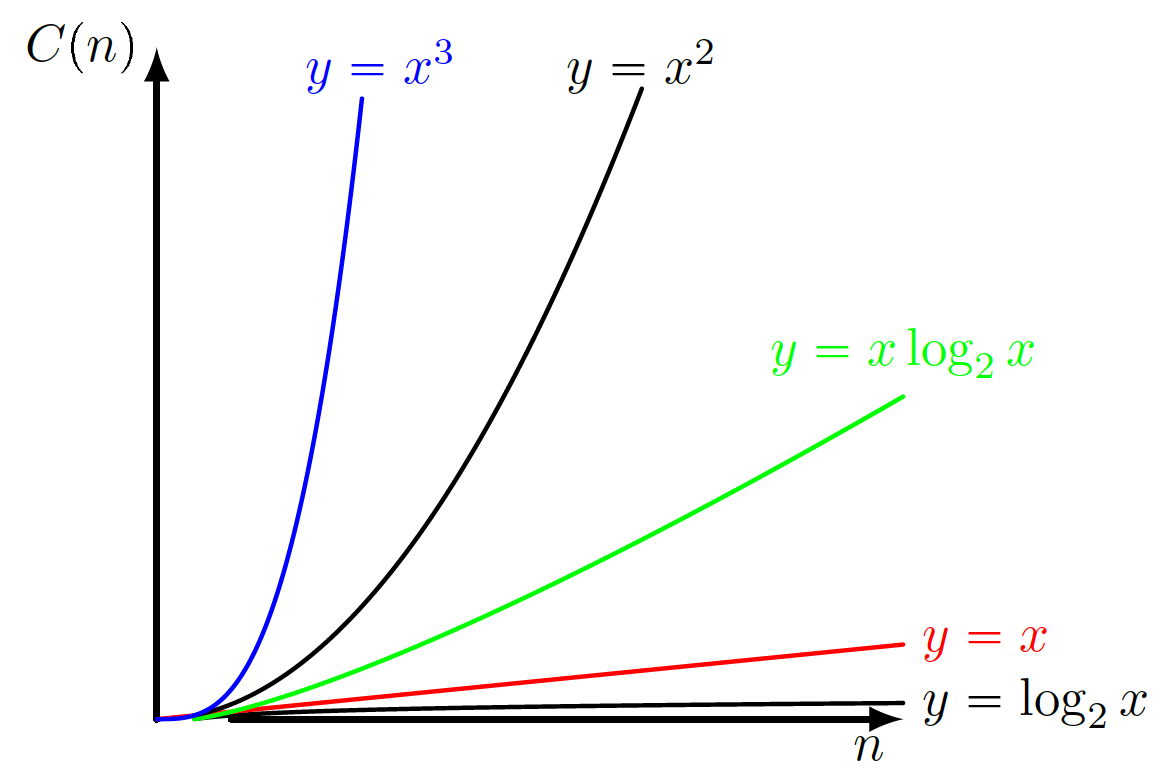
\includegraphics[width=0.8\textwidth]{002_Complexite.png}
	\end{figure}
	
	
			
	\pagebreak
	\section{Algorithmes de tri}
	

\end{document}


%Eléments manquants:
